\begin{figure}[H]
\centering
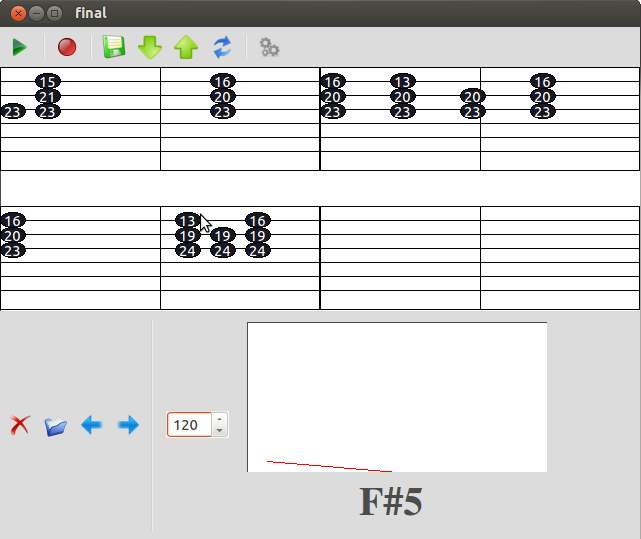
\includegraphics[scale=0.5]{RenduFinal}
\caption{Rendu final de l'application}
\end{figure}



\paragraph{}
Afin de lier l'application cliente et l'application web, nous utilisons un format de sauvegarde partagé par les deux 
langages (C++ et JS), le JSON. Nous avons donc conçu un simple parser JSON afin de pouvoir sauvegarder une partition 
soit sur son PC local, soit dans la base de donnée distante pour la partager avec le monde. Nous avons choisi 
ce format d'enregistrement car il est aisément lisible sur le serveur qui peut alors traiter rapidement les informations 
pour les afficher au utilisateurs, et car c'est un format de plus en plus répandu. Nous aurions pu prendre du XML, mais 
il aurait été moins bien traité côté serveur. De plus, le format JSON consomme moins de place en mémoire que le format XML,
car il est légèrement moins verbeux. L'application possède donc des fonctionnalités de sauvegardes sous forme de fichier et 
de sauvegarde sur le \"cloud\" representé par le site web. Il est possible de réouvrir une partition sauvegardée en local.

\paragraph{}
La bibliothèque FMOD Ex nous permet de récupérer le son entrant de l'application. Elle a été choisi car elle est simple 
d'utilisation tout en étant efficace. Cela nous a permis de nous concentrer sur le traitement de ce son, qui constitue 
une des parties les plus importante du projet. Nous avons suivi l'algorithme du rapport de conception, et y avons apporté 
quelques modifications pour l'implémentation réelle. Cet algorithme permet de récupérer les notes ayant le volume le plus 
élevé capté par le micro. Nous pouvons également définir une plage de fréquences afin d'enlever tout parasite possible. Par exemple, 
dans le cas de la guitare, nous pouvons filtrer toutes les notes qui ne peuvent pas être jouée avec une guitare. 

\paragraph{}
La bibliothèque Qt ne crée pas de nouveau thread pour sa partie graphique comme Swing par exemple, nous avons donc du créer deux nouveaux 
thread pour l'enregistrement de partitions et l'accordeur. Il a été aisé d'implementer ces thread car Qt nous permet d'en 
faire un héritant d'une de ses classes. Sans ces threads, l'applications serait par exemple bloquée si l'on appuie sur le 
bouton d'enregistrement, car celui ne serait plus accessible une fois l'enregistrement lancé.

\paragraph{}
La quantité de fréquences a traiter étant importante (8192 tous les pas de temps), nous avons décidé d'utiliser 
le tri rapide pour un maximum de performance. Nous avons due y ajouter une surcouche sauvegardant les places de chaque fréquences 
car FMOD assigne chaque volume de fréquence à sa place dans le tableau. Si nous avions uniquement trié le tableau de fréquences 
en fonction du volume, nous n'aurions plus la possibilité de savoir quelle fréquence a le volume le plus haut. Nous avons choisi 
ce nombre de fréquences à traiter car c'est le maximum proposé par FMOD, et ce nombre nous permet donc d'avoir le maximum de 
précision possible pour le traitement des fréquences.

\paragraph{}
Nous avons choisi de fournir deux classes sous le design pattern du singleton car cela simplifiait beaucoup le développement, et 
car plusieurs instances de ces deux classes serait inutiles. La classe Notes fournit donc toutes les notes possiblement enregistrable 
dans la musique, et la classe Guitar fournit la possibilité de convertir les notes jouées en frettes pour permettre l'affichage de la 
tablature. Nous nous sommes donc plus concentré sur les tablatures pour guitare et non les partitions en général, 
mais il serait possible de l'adapter pour tous les instrument. Il est également possible de changer l'accordage de la guitare, mais 
uniquement en changeant le code, faute d'un manque de temps pour développer cette fonctionnalité.

\paragraph{}
Le pattern MVC n'existant pas en C++, nous avons créé une classe NoSkin correspondant à l'affichage graphique, une classe Partition représentant le modèle de l'application et une classe Controller afin de rester au plus proche de cette méthode de conception. \\
Ceci nous a permis de nous répartir les tâches de manière optimale et de lier nos parties respectives en évitant la majorité des complications. La liaison 
entre le modèle, le controlleur et la vue se fait principalement dans la classe Controller. En effet, celle ci comporte des attributs appartenant aux autres 
parties. A l'exception dans la classe TuneThread qui comporte des attributs graphiques, car cette classe doit mettre à jour en temps réel l'accordeur 
sous forme graphique. La gestion des évènements permet de plus de faire une liaison aisée entre modèle et vue. Les slots sont appelés grâce aux 
élements graphique de la vue, ce qui entraîne des appels de méthodes du modèle, tout en mettant à jour la vue par la suite. 

\paragraph{}
En ce qui concerne la classe graphique principale NoSkin, on y a implanté les éléments nécessaires à l'interface graphique et on lui a assigné un layout de base, tout en considérant le fait que par la suite on pourrait hériter de cette classe pour permettre des interfaces plus personnalisées.

\paragraph{}
Pour faciliter sa connexion, l'utilisateur peut enregistrer ses données de connexion à partir de l'application en les enregistrant dans le fichier 
\"user.conf\". Il peut ainsi se connecter automatiquement lorsqu'il souhaite uploader ou télécharger une de ses partitions. La fenêtre de configuration 
a été prévue pour y ajouter d'autres fonctionnalités de configuration de l'application, comme par exemple la personnalisation de l'aspect graphique ou 
plus simplement le tempo initial d'une partition à sa création ou a l'ouverture du logiciel.



\begin{figure}[H]
\centering
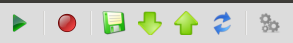
\includegraphics[scale=0.5]{TopApp}
\caption{Barre de menu haut}
\end{figure}
\paragraph{}
Voici la description des boutons dans leur ordre d'apparition de droite à gauche:\\
- Bouton play\\
Permet de jouer une partition pour voir le rendu de la composition effectuée\\
- Bouton record\\
Permet de lancer l'enregistrement de la partition. Il se change en un bouton stop au premier appuie. Si on appuie à nouveau dessus, 
l'enregistrement s'arrêtera.\\
- Bouton save\\
Permet d'ouvrir le selecteur de fichier pour sauvegarder la partition. Si elle a déjà été sauvegardé, elle sera directement sauvegarder sans 
ouvrir à nouveau le selecteur de fichier.\\
- Bouton download\\
Ouvre le selecteur de partitions stockées sur le site web afin de les télécharger et de les avoir en local.\\
- Bouton upload\\
Upload sur le site web la partition courante. Si cette partition n'a pas de nom, alors l'application ouvrira une boite de dialogue pour permettre 
l'entrée de l'utilisateur.\\
- Bouton connection\\
Permet de se connecter au site web avec les informations fournis dans la configuration. La connexion est automatique lorsqu'on download 
ou lorqu'on upload une partition.\\
- Bouton configuration\\
Ouvre la fenêtre de configuration permettant de rentrer ses informations de connexion ou ses préférences pour l'application.\\


\begin{figure}[H]
\centering
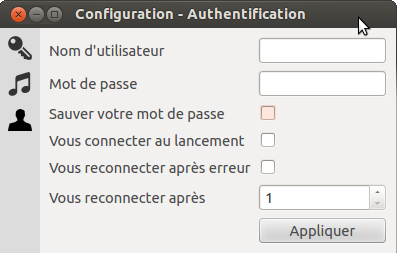
\includegraphics[scale=0.5]{Config}
\caption{Fenêtre de configuration}
\end{figure}
La fenêtre de configuration permet comme indiqué ci dessus de rentrer ses identifiants pour se connecter à la base de données et ainsi 
intéragir avec le serveur de stockage a distance des ses partitions.

\begin{figure}[H]
\centering
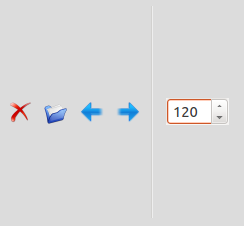
\includegraphics[scale=0.5]{BotApp}
\caption{Barre de menu basse}
\end{figure}
\paragraph{}
Voici la description des boutons dans leur ordre d'apparition de droite à gauche:\\
- Bouton delete\\
Permet de supprimer la partition en cours. Si elle n'a pas été sauvegardé, une boite de dialogue s'ouvre pour demander si l'utilisateur 
veut la sauvegarder ou non. Ce bouton efface donc toutes les notes de la partition.\\
- Bouton open\\
Permet d'ouvrir une partition qui a été sauvegardée sur la machine local. Ce bouton ouvre un selecteur de fichier pour choisir le fichier 
voulu. Si une erreur de produit lors de la lecture, rien de ne passera.\\
- Bouton left\\
Permet de déplacer l'affichage vers le début de la partition.\\
- Bouton right\\
Permet de déplacer l'affichage vers la fin de la partition.\\
- Selecteur tempo\\
Permet de modifier le tempo de la partition. Ce tempo est effectif dans la sauvegarde de la partition, son enregistrement ainsi que sa lecture.
\begin{figure}[H]
\centering
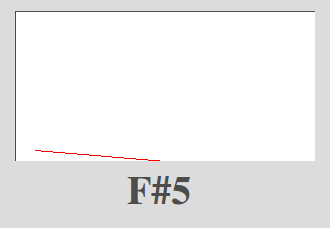
\includegraphics[scale=0.5]{Tuner}
\caption{Accordeur intégré}
\end{figure}
L'accordeur intégré permet d'accorder à tout moment son instrument pour être sur de jouer juste. Une guitare parfaitement accordée permettra donc 
de faire un enregistrement de partition plus précis. L'accordeur affiche la note captée la plus proche et indique dans quel sens l'utilisateur 
doit accorder la corde jouée.

\begin{figure}[H]
\centering
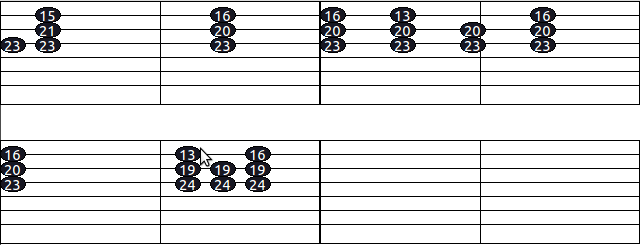
\includegraphics[scale=0.5]{Part}
\caption{Affichage d'une partition}
\end{figure}
Voici la partie principale de l'application, l'affichage de la partition. L'affichage fonctionne sur le même principe que les tablatures ou les 
partitions et la note de la corde la plus grave se trouve le plus en bas. Le chiffre affiché est le numéro de la frette à jouer sur la guitare pour 
produire la même note. On peut distinctement voir les accords, composés de plusieurs notes alignées verticalement.